% !TeX program = lualatex
% ================================================================
% Polish Parallel Text Version of ProbabilityRevision
%
% Generated by the server using the following settings:
%
%   language            Polish (pol)
%   text direction      left to right
%   font                Noto Serif
%   fallback font       Noto Serif
%   built from          latex/worksheets/revision/probabilityRevision.tex
%   vocabulary key      latex/worksheets/revision/probabilityRevision/L2/pol/probabilityRevision_polishKey.tex
%   tier 3 vocabulary   green   RGB 0 128 0
%   English text        black   RGB 0 0 0
%   Polish text         purple  RGB 112 48 160
%   layout macros       version 3
%
% Please don't edit any information in this comment block - the server
% compares it against the current settings and rebuilds this file when
% they differ, so changes here would be overwritten. However, feel free
% to make updates to the LaTeX below if you want to edit it.
% ================================================================

\documentclass[11pt,a4paper]{article}
% ================================================================
% Copied from the English sheet this was translated from, so that
% anything it sets up for itself still works here
% ================================================================
\usepackage[a4paper,top=14mm,bottom=14mm,left=15mm,right=15mm]{geometry}
\usepackage[T1]{fontenc}
\usepackage{amsmath}
\usepackage{amssymb}
\usepackage{array}
\usepackage{multicol}
\usepackage{tikz}
\usetikzlibrary{arrows.meta}

% ================================================================
% Probability: revision questions.
%
% Two pages of questions, in black and white, with a heading for each
% topic on the Maths Revision topic list in the same order. Each topic
% has a few short questions that start easy, with a diagram only where
% a question uses one, and the sheet ends with some problem solving.
% There are no key facts or worked examples on the sheet: the methods
% are in the worked solutions and the revision guide. Questions are
% numbered through the sheet so that the answer key and the worked
% solutions can refer to them.
% ================================================================

\pagestyle{empty}
\setlength{\parindent}{0pt}
\setlength{\parskip}{2pt}
\setlength{\columnsep}{9mm}

% A topic from the revision list.
\newcommand{\topic}[1]{\par\addvspace{9pt}{\bfseries #1}\par\nobreak\vspace{2pt}}

% Questions are numbered through the whole sheet.
\newcounter{qn}
\newcommand{\q}{\par\addvspace{5pt}\stepcounter{qn}\hangindent=1.6em\hangafter=1\noindent
  \makebox[1.6em][l]{\textbf{\theqn}}}

% \venn{<left set>}{<right set>}{<left only>}{<both>}{<right only>}{<outside>}
% The last argument is drawn as it stands, to place the outside
% region's contents anywhere around the circles.
\newcommand{\venn}[6]{%
  \begin{tikzpicture}[x=1mm,y=1mm]
    \draw (0,0) rectangle (66,34);
    \node[anchor=north west] at (0,34) {$\xi$};
    \draw (24,17) circle (13.5);
    \draw (42,17) circle (13.5);
    \node at (10,30) {$#1$};
    \node at (56,30) {$#2$};
    \node[align=center] at (17.5,17) {#3};
    \node[align=center] at (33,17) {#4};
    \node[align=center] at (48.5,17) {#5};
    #6
  \end{tikzpicture}}

% \freqtree{<total>}{<group>}{<n>}{<group>}{<n>}{<leaf>}{<leaf>}{<leaf>}{<leaf>}
% A frequency tree drawn left to right. The two outcomes on the right
% hand branches are named by \leafa and \leafb.
\newcommand{\leafa}{}
\newcommand{\leafb}{}
\newcommand{\freqtree}[9]{%
  \begin{tikzpicture}[x=1mm,y=1mm,
      box/.style={draw,minimum width=9mm,minimum height=5.5mm,inner sep=1pt},
      lab/.style={font=\small,inner sep=1pt}]
    \node[box] (r) at (0,0) {#1};
    \node[box] (u) at (18,10) {#3};
    \node[lab,above] at (u.north) {#2};
    \node[box] (d) at (18,-10) {#5};
    \node[lab,below] at (d.south) {#4};
    \node[box] (uu) at (37,14.5) {#6};
    \node[box] (ud) at (37,5.5) {#7};
    \node[box] (du) at (37,-5.5) {#8};
    \node[box] (dd) at (37,-14.5) {#9};
    \foreach \n in {uu,du}{\node[lab,right] at (\n.east) {\leafa};}
    \foreach \n in {ud,dd}{\node[lab,right] at (\n.east) {\leafb};}
    \draw (r.east) -- (u.west) (r.east) -- (d.west);
    \draw (u.east) -- (uu.west) (u.east) -- (ud.west);
    \draw (d.east) -- (du.west) (d.east) -- (dd.west);
  \end{tikzpicture}}

% Characters this language's font has not got are borrowed from another,
% rather than being silently dropped - see docs/translated-sheet-latex.md
\directlua{%
  if luaotfload and luaotfload.add_fallback then
    luaotfload.add_fallback("eallatinfallback",
      { "Noto Serif:mode=harf;" })
  else
    tex.error("this luaotfload is too old to register a fallback font")
  end
}
\usepackage[english]{babel}
\babelprovide[import]{polish}
\babelfont[polish]{rm}[Renderer=Harfbuzz, BoldFont={Noto Serif}, ItalicFont={Noto Serif}, BoldItalicFont={Noto Serif}, RawFeature={fallback=eallatinfallback}]{Noto Serif}
\babelfont[polish]{sf}[Renderer=Harfbuzz, BoldFont={Noto Serif}, ItalicFont={Noto Serif}, BoldItalicFont={Noto Serif}, RawFeature={fallback=eallatinfallback}]{Noto Serif}
\newcommand{\ealtext}[1]{\foreignlanguage{polish}{#1}}
\newcommand{\ealtextblock}[1]{{\raggedright\foreignlanguage{polish}{#1}\par}}
% ================================================================
% EAL layout helpers
% ================================================================
\usepackage{xcolor}

\definecolor{ealkeycolour}{RGB}{0,128,0}
\definecolor{ealenglish}{RGB}{0,0,0}
\definecolor{ealtwocolour}{RGB}{112,48,160}

\newsavebox{\ealboxen}
\newsavebox{\ealboxtr}
\newlength{\ealglosswd}
\newlength{\ealglossraise}
\setlength{\ealglossraise}{1.15em}

% a tier 3 word, in English and in translation alike
\newcommand{\ealkey}[1]{\textcolor{ealkeycolour}{#1}}
\newcommand{\ealkeytr}[1]{\textcolor{ealkeycolour}{\ealtext{#1}}}

% One translated word above one English word. Built from kernel
% primitives, never a tabular, which would break wherever the sheet
% loads array, booktabs or tabularx. The box is as wide as the wider of
% the two, so a long translation pushes its neighbours aside instead of
% overlapping them, and it claims its full height so a table row or a
% TikZ node makes room for it.
\newcommand{\ealgloss}[2]{%
  \sbox{\ealboxen}{\ealkey{#1}}%
  \sbox{\ealboxtr}{\small\textcolor{ealtwocolour}{\ealtext{#2}}}%
  \setlength{\ealglosswd}{\wd\ealboxen}%
  \ifdim\wd\ealboxtr>\ealglosswd\setlength{\ealglosswd}{\wd\ealboxtr}\fi
  \leavevmode
  \makebox[\ealglosswd][c]{%
    \makebox[0pt][c]{\usebox{\ealboxen}}%
    \makebox[0pt][c]{\raisebox{\ealglossraise}{\usebox{\ealboxtr}}}%
  }%
}

% opens up line spacing around a block of glosses, so the raised
% translations sit clear of the line above
\newenvironment{ealglossed}{\par\linespread{2.1}\selectfont\ignorespaces}{\par}

% a whole translated sentence above its English counterpart. block level,
% so it does not belong inside a tabular cell
\newcommand{\ealpara}[2]{%
  \par\addvspace{0.5\baselineskip}%
  {\color{ealtwocolour}\ealtextblock{#1}}%
  \penalty200
  {\color{ealenglish}#2\par}%
  \addvspace{0.5\baselineskip}%
}

\begin{document}
% Ragged right, without \raggedright, which would make \\ end the
% paragraph and lose the hanging indent of a question's later lines.
\setlength{\rightskip}{0pt plus 4em}

{\Large\bfseries \ealkey{Probability}}\hfill{\large Revision questions}
\par\vspace{2pt}\hrule\vspace{4pt}

\begin{multicols}{2}

% ----------------------------------------------------------------
\ealpara{Zapisywanie \ealkeytr{prawdopodobieństw} jako \ealkeytr{ułamków}, \ealkeytr{ułamków dziesiętnych} i \ealkeytr{procentów}.}{Writing \ealkey{probabilities} as \ealkey{fractions}, \ealkey{decimals} and \ealkey{percentages}}
\topic{Writing \ealkey{probabilities} as \ealkey{fractions}, \ealkey{decimals} and \ealkey{percentages}}
\q \ealpara{W torbie jest 4 zielone (G), 6 żółtych (Y) i 10 białych (W) cukierków. Jeden cukierek jest wybierany \ealkeytr{losowo}. Zapisz P(green) jako \ealkeytr{ułamek}, \ealkeytr{ułamek dziesiętny} i \ealkeytr{procent}.}{A bag holds 4 green (G), 6 yellow (Y) and 10 white (W) sweets. One sweet is taken at \ealkey{random}. Write P(green) as a \ealkey{fraction}, a \ealkey{decimal} and a \ealkey{percentage}.}
\par\vspace{4pt}
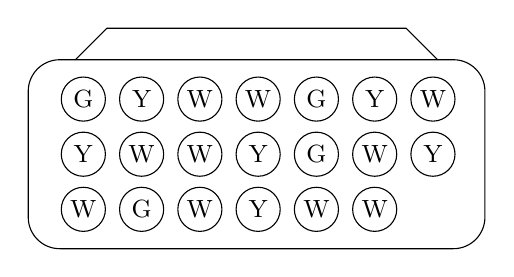
\begin{tikzpicture}[x=1mm,y=1mm]
  \draw[rounded corners=4mm] (0,0) rectangle (58,24);
  \draw (6,24) -- (10,28) -- (48,28) -- (52,24);
  \foreach \l [count=\i from 0] in {G,Y,W,W,G,Y,W,Y,W,W,Y,G,W,Y,W,G,W,Y,W,W}{
    \pgfmathtruncatemacro{\r}{\i/7}
    \pgfmathtruncatemacro{\c}{mod(\i,7)}
    \draw (7+\c*7.4,19-\r*7) circle (2.8);
    \node[font=\small] at (7+\c*7.4,19-\r*7) {\l};}
\end{tikzpicture}
\q \ealpara{\ealkeytr{Prawdopodobieństwo}, że pociąg się spóźni, wynosi 0.12. Jakie jest \ealkeytr{prawdopodobieństwo}, że się nie spóźni?}{The \ealkey{probability} that a train is late is 0.12. What is the \ealkey{probability} that it is not late?}
\q \ealpara{Tabela pokazuje \ealkeytr{prawdopodobieństwa}, że spinner wskaże każdy kolor. Znajdź \ealkeytr{prawdopodobieństwo}, że wskaże żółty.}{The table shows the \ealkey{probabilities} of a spinner landing on each colour. Find the \ealkey{probability} that it lands on yellow.}
\par\vspace{4pt}
{\renewcommand{\arraystretch}{1.5}%
\begin{tabular}{|l|c|c|c|c|}\hline
Colour & Red & Blue & Green & Yellow\\\hline
\ealkey{Probability} & 0.3 & 0.25 & 0.15 & \\\hline
\end{tabular}}

% ----------------------------------------------------------------
\ealpara{Systematyczne wypisywanie \ealkeytr{wyników}.}{Listing \ealkey{outcomes} systematically}
\topic{Listing \ealkey{outcomes} systematically}
\q \ealpara{Kawiarnia sprzedaje trzy przystawki: zupę (S), melon (M) i krewetki (P). Sprzedaje dwa dania główne: rybę (F) i curry (C). Wypisz wszystkie możliwe zestawy jednej przystawki i jednego dania głównego.}{A caf\'e sells three starters: soup (S), melon (M) and prawns (P). It sells two mains: fish (F) and curry (C). List all the possible meals of one starter and one main.}
\q \ealpara{Spinner A ma numery 1, 2, 3, 4. Spinner B ma numery 1, 2, 3. Oboma spinnerami się kręci, a otrzymane liczby są mnożone.}{Spinner A is numbered 1, 2, 3, 4. Spinner B is numbered 1, 2, 3. Both spinners are spun, and the two scores are multiplied.}
\ealpara{(a) Skopiuj i uzupełnij \ealkeytr{diagram przestrzeni prób}.}{(a) Copy and complete the \ealkey{sample space diagram}.}
\ealpara{(b) Znajdź \ealkeytr{prawdopodobieństwo}, że odpowiedź jest \ealkeytr{parzysta}.}{(b) Find the \ealkey{probability} that the answer is \ealkey{even}.}
\par\vspace{4pt}
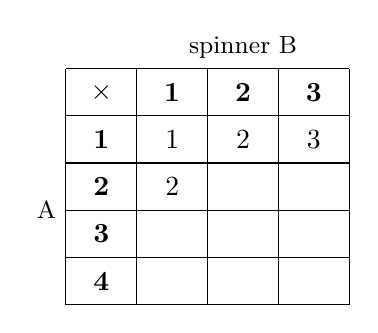
\begin{tikzpicture}[x=9mm,y=6mm]
  \draw[step={(1,1)}] (0,-4) grid (4,1);
  \node at (0.5,0.5) {$\times$};
  \foreach \b in {1,2,3}{\node at (\b+0.5,0.5) {\textbf{\b}};}
  \foreach \a in {1,...,4}{\node at (0.5,-\a+0.5) {\textbf{\a}};}
  \foreach \b in {1,2,3}{\node at (\b+0.5,-0.5) {\b};}
  \node at (1.5,-1.5) {2};
  \node[above] at (2.5,1) {\small spinner B};
  \node[left] at (0,-2) {\small A};
\end{tikzpicture}

% ----------------------------------------------------------------
\ealpara{Oczekiwane rezultaty.}{Expected results}
\topic{Expected results}
\q \ealpara{\ealkeytr{Uczciwą} monetą rzuca się 300 razy. Ile orłów oczekiwałbyś?}{A \ealkey{fair} coin is flipped 300 times. How many heads would you expect?}
\q \ealpara{\ealkeytr{Prawdopodobieństwo}, że autobus się spóźni, wynosi 0.08. Na ilu z 250 podróży oczekiwałbyś, że autobus się spóźni?}{The \ealkey{probability} that a bus is late is 0.08. On how many of 250 journeys would you expect the bus to be late?}

% ----------------------------------------------------------------
\ealpara{\ealkeytr{Prawdopodobieństwo doświadczalne}.}{\ealkey{Experimental probability}}
\topic{\ealkey{Experimental probability}}
\q \ealpara{Kostką rzuca się 200 razy. Tabela pokazuje rezultaty.}{A dice is rolled 200 times. The table shows the results.}
\par\vspace{4pt}
{\renewcommand{\arraystretch}{1.5}%
\begin{tabular}{|l|c|c|c|c|c|c|}\hline
Score & 1 & 2 & 3 & 4 & 5 & 6\\\hline
\ealkey{Frequency} & 31 & 35 & 30 & 36 & 33 & 35\\\hline
\end{tabular}}
\par\vspace{4pt}
\ealpara{(a) Znajdź \ealkeytr{częstość względną} wyrzucenia 4.}{(a) Find the \ealkey{relative frequency} of rolling a 4.}
\ealpara{(b) Czy rezultaty sugerują, że kostka jest \ealkeytr{uczciwa}? Wyjaśnij swoją odpowiedź.}{(b) Do the results suggest that the dice is \ealkey{fair}? Explain your answer.}
\q \ealpara{Jo rzuca monetą 20 razy i otrzymuje 14 orłów. Kai rzuca tą samą monetą 500 razy i otrzymuje 260 orłów. Czyje rezultaty dają lepsze oszacowanie \ealkeytr{prawdopodobieństwa} orła? Zapisz to oszacowanie.}{Jo flips a coin 20 times and gets 14 heads. Kai flips the same coin 500 times and gets 260 heads. Whose results give the better estimate of the \ealkey{probability} of heads? Write down this estimate.}

% ----------------------------------------------------------------
\ealpara{\ealkeytr{Drzewka częstości}.}{\ealkey{Frequency trees}}
\topic{\ealkey{Frequency trees}}
\q \ealpara{120 osób odwiedziło muzeum. 70 z nich było dorosłych. 45 dorosłych kupiło przewodnik. 20 dzieci kupiło przewodnik.}{120 people visited a museum. 70 of them were adults. 45 of the adults bought a guidebook. 20 of the children bought a guidebook.}
\ealpara{(a) Skopiuj i uzupełnij \ealkeytr{drzewko częstości}.}{(a) Copy and complete the \ealkey{frequency tree}.}
\ealpara{(b) Odwiedzający jest wybierany \ealkeytr{losowo}. Znajdź \ealkeytr{prawdopodobieństwo}, że kupił przewodnik.}{(b) A visitor is chosen at \ealkey{random}. Find the \ealkey{probability} that they bought a guidebook.}
\par\vspace{4pt}
{\renewcommand{\leafa}{Book}\renewcommand{\leafb}{No book}%
\freqtree{120}{Adults}{}{Children}{}{}{}{}{}}

\end{multicols}

\newpage

\begin{multicols}{2}

% ----------------------------------------------------------------
\ealpara{\ealkeytr{Diagramy Venna}.}{\ealkey{Venn diagrams}}
\topic{\ealkey{Venn diagrams}}
\q \ealpara{W roczniku jest 50 uczniów. 28 uczy się francuskiego (F), 19 uczy się hiszpańskiego (S), a 8 uczy się obu.}{There are 50 pupils in a year group. 28 study French (F), 19 study Spanish (S), and 8 study both.}
\ealpara{(a) Skopiuj i uzupełnij \ealkeytr{diagram Venna}.}{(a) Copy and complete the \ealkey{Venn diagram}.}
\ealpara{(b) Uczeń jest wybierany \ealkeytr{losowo}. Znajdź \ealkeytr{prawdopodobieństwo}, że nie uczy się żadnego z tych języków.}{(b) A pupil is chosen at \ealkey{random}. Find the \ealkey{probability} that they study neither language.}
\par\vspace{4pt}
\venn{F}{S}{}{}{}{}
\q \ealpara{\ealkeytr{Diagram Venna} pokazuje liczby od 1 do 15. A to liczby \ealkeytr{parzyste}, a B to \ealkeytr{liczby kwadratowe}. Jedna z liczb jest wybierana \ealkeytr{losowo}. Znajdź}{The \ealkey{Venn diagram} shows the numbers from 1 to 15. A is the \ealkey{even} numbers and B is the \ealkey{square numbers}. One of the numbers is chosen at \ealkey{random}. Find}
\ealpara{(a) P($A\cap B$), \ealkeytr{prawdopodobieństwo}, że należy do A i B}{(a) P($A\cap B$), the \ealkey{probability} that it is in A and B}
\ealpara{(b) P($A\cup B$), \ealkeytr{prawdopodobieństwo}, że należy do A lub B lub do obu}{(b) P($A\cup B$), the \ealkey{probability} that it is in A or B or both}
\ealpara{(c) P($A'$), \ealkeytr{prawdopodobieństwo}, że nie należy do A.}{(c) P($A'$), the \ealkey{probability} that it is not in A.}
\par\vspace{4pt}
\venn{A}{B}{\hspace*{2mm}2\enspace 6\\[1pt]\hspace*{2mm}8\enspace 10\\[1pt]\hspace*{2mm}12\enspace 14}{4}{1\\[2pt]9}%
  {\node at (4,17) {3}; \node at (62,17) {5}; \node at (4,4) {7}; \node at (62,4) {11};
   \node at (33,31.3) {13}; \node at (33,2.7) {15};}

% ----------------------------------------------------------------
\ealpara{\ealkeytr{Prawdopodobieństwo warunkowe} z \ealkeytr{diagramami Venna}.}{\ealkey{Conditional probability} with \ealkey{Venn diagrams}}
\topic{\ealkey{Conditional probability} with \ealkey{Venn diagrams}}
\q \ealpara{\ealkeytr{Diagram Venna} pokazuje 60 osób i informację, czy mają kota (C) czy psa (D).}{The \ealkey{Venn diagram} shows 60 people, and whether they own a cat (C) or a dog (D).}
\par\vspace{4pt}
\venn{C}{D}{14}{10}{21}{\node at (60,4) {15};}
\par\vspace{2pt}
\ealpara{(a) Znajdź \ealkeytr{prawdopodobieństwo}, że wybrana \ealkeytr{losowo} osoba ma psa.}{(a) Find the \ealkey{probability} that a person chosen at \ealkey{random} owns a dog.}
\ealpara{(b) \ealkeytr{Pod warunkiem, że} osoba ma psa, znajdź \ealkeytr{prawdopodobieństwo}, że ma także kota.}{(b) \ealkey{Given} that a person owns a dog, find the \ealkey{probability} that they also own a cat.}
\q \ealpara{Użyj swojego \ealkeytr{diagramu Venna} z pytania 11. \ealkeytr{Pod warunkiem, że} uczeń uczy się francuskiego, znajdź \ealkeytr{prawdopodobieństwo}, że uczy się także hiszpańskiego.}{Use your \ealkey{Venn diagram} from question 11. \ealkey{Given} that a pupil studies French, find the \ealkey{probability} that they also study Spanish.}

% ----------------------------------------------------------------
\ealpara{Rozwiązywanie problemów.}{Problem solving}
\topic{Problem solving}
\q \ealpara{W torbie są czerwone i niebieskie żetony w \ealkeytr{stosunku} $3:5$. Do torby wkłada się dwa dodatkowe czerwone żetony. Teraz \ealkeytr{prawdopodobieństwo} wylosowania czerwonego żetonu wynosi $\frac12$. Ile żetonów było w torbie na początku?}{A bag holds red and blue counters in the \ealkey{ratio} $3:5$. Two more red counters are put in the bag. Now the \ealkey{probability} of taking a red counter is $\frac12$. How many counters were in the bag at the start?}
\q \ealpara{Spinner ma 5 równych sekcji, każda pokolorowana na czerwono, niebiesko lub zielono. \ealkeytr{Prawdopodobieństwo} czerwonego wynosi 0.4, a \ealkeytr{prawdopodobieństwo} niebieskiego jest dwa razy większe niż \ealkeytr{prawdopodobieństwo} zielonego. Narysuj spinner.}{A spinner has 5 equal sections, each coloured red, blue or green. The \ealkey{probability} of red is 0.4, and the \ealkey{probability} of blue is twice the \ealkey{probability} of green. Draw the spinner.}
\q \ealpara{Sam rzuca kostką 6 razy i ani razu nie wyrzuca 6. Mówi: „Kostka musi być \ealkeytr{obciążona}”. Czy Sam ma rację? Wyjaśnij swoją odpowiedź.}{Sam rolls a dice 6 times and never gets a 6. He says, ``The dice must be \ealkey{biased}.'' Is Sam right? Explain your answer.}

\end{multicols}

\end{document}